From the analyse of the results of the measurements in Appedix XX, it is shown, that the height of the antennas and the distance between them have a much higher influence on the PL, than the other parameter, which is the placement, antenna type and polarization. As these parameters have much less influence on the PL, there will only be looking at the different height combinations and distance between the antennas.

Firstly there will be looked at the case, where the height of the transmitting antenna and the receiving antenna is at the same heights, over the different distance.

\begin{figure}
\centering
% This file was created by matlab2tikz.
%
%The latest updates can be retrieved from
%  http://www.mathworks.com/matlabcentral/fileexchange/22022-matlab2tikz-matlab2tikz
%where you can also make suggestions and rate matlab2tikz.
%
\definecolor{mycolor1}{rgb}{0.00000,0.44700,0.74100}%
\definecolor{mycolor2}{rgb}{0.85000,0.32500,0.09800}%
\definecolor{mycolor3}{rgb}{0.92900,0.69400,0.12500}%
\definecolor{mycolor4}{rgb}{0.49400,0.18400,0.55600}%
%
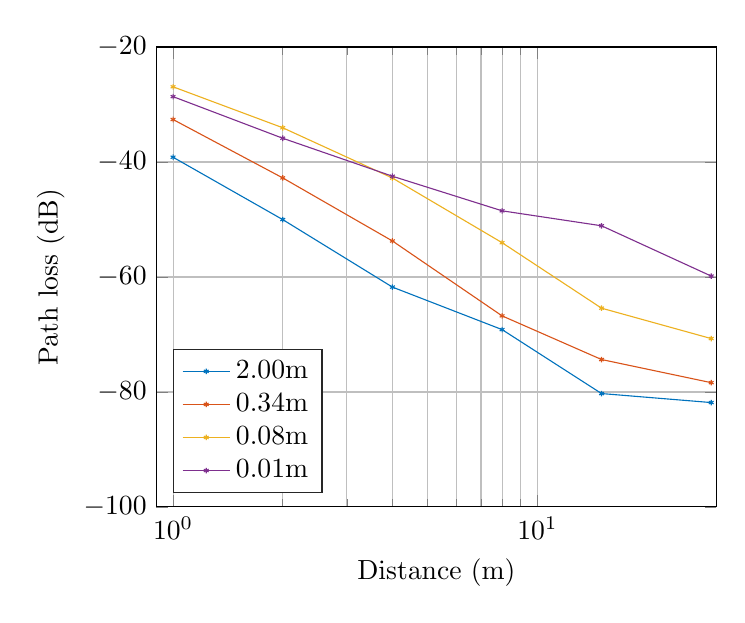
\begin{tikzpicture}

\begin{axis}[%
width=2.8in,
height=2.3in,
at={(2.08in,0.858in)},
scale only axis,
xmode=log,
xmin=0.9,
xmax=31,
xlabel=Distance (m),
xminorticks=true,
xmajorgrids,
xminorgrids,
ymin=-100,
ymax=-20,
ylabel=Path loss (dB),
ymajorgrids,
legend pos = south west,
axis background/.style={fill=white},
legend style={legend cell align=left,align=left,draw=white!15!black}
]
\addplot [color=mycolor1,solid,mark size=1.0pt,mark=asterisk,mark options={solid}]
  table[row sep=crcr]{%
1	-39.176832441447\\
2	-50.0236813268286\\
4	-61.7627349006033\\
8	-69.1568155321866\\
15	-80.2784721484843\\
30	-81.8463231335614\\
};
\addlegendentry{2.00m};

\addplot [color=mycolor2,solid,mark size=1.0pt,mark=asterisk,mark options={solid}]
  table[row sep=crcr]{%
1	-32.6162301822822\\
2	-42.7733202106742\\
4	-53.7406598744587\\
8	-66.7692891298477\\
15	-74.3619892107941\\
30	-78.384604174472\\
};
\addlegendentry{0.34m};

\addplot [color=mycolor3,solid,mark size=1.0pt,mark=asterisk,mark options={solid}]
  table[row sep=crcr]{%
1	-26.9292301822822\\
2	-34.0517673842044\\
4	-42.7927848744587\\
8	-54.0404141298477\\
15	-65.4297392107941\\
30	-70.718229174472\\
};
\addlegendentry{0.08m};

\addplot [color=mycolor4,solid,mark size=1.0pt,mark=asterisk,mark options={solid}]
  table[row sep=crcr]{%
1	-28.6391813268286\\
2	-35.8754849006033\\
4	-42.4804405321866\\
8	-48.4989721484843\\
15	-51.0989481335614\\
30	-59.847479174472\\
};
\addlegendentry{0.01m};

\end{axis}
\end{tikzpicture}%
\caption{Mesurements of PL for transmitter and receiver antenna at the same height.}
\label{Meas1}
\end{figure}

It is seen on figure \ref{Meas1}, that the longer the distance, the higher the PL. This comes from the same principle, that the Friss model is based on. When looking at the graph compared to changing the heights, it is seen, that the lower the antennas is placed, the higher PL. This comes from the principle, that reflections comes from the ground and comes with (in most cases) destructive interference, which the Two Ray model is based on. 

Secondly there will be looked at the case, where the height of the transmitting antenna is kept at a single height, both low at 0.01m (Figure \ref{Meas2}) and high at 2.00m (Figure \ref{Meas3}), while the height of the receiving antenna is varying.

\begin{figure}
\centering
% This file was created by matlab2tikz.
%
%The latest updates can be retrieved from
%  http://www.mathworks.com/matlabcentral/fileexchange/22022-matlab2tikz-matlab2tikz
%where you can also make suggestions and rate matlab2tikz.
%
\definecolor{mycolor1}{rgb}{0.00000,0.44700,0.74100}%
\definecolor{mycolor2}{rgb}{0.85000,0.32500,0.09800}%
\definecolor{mycolor3}{rgb}{0.92900,0.69400,0.12500}%
\definecolor{mycolor4}{rgb}{0.49400,0.18400,0.55600}%
%
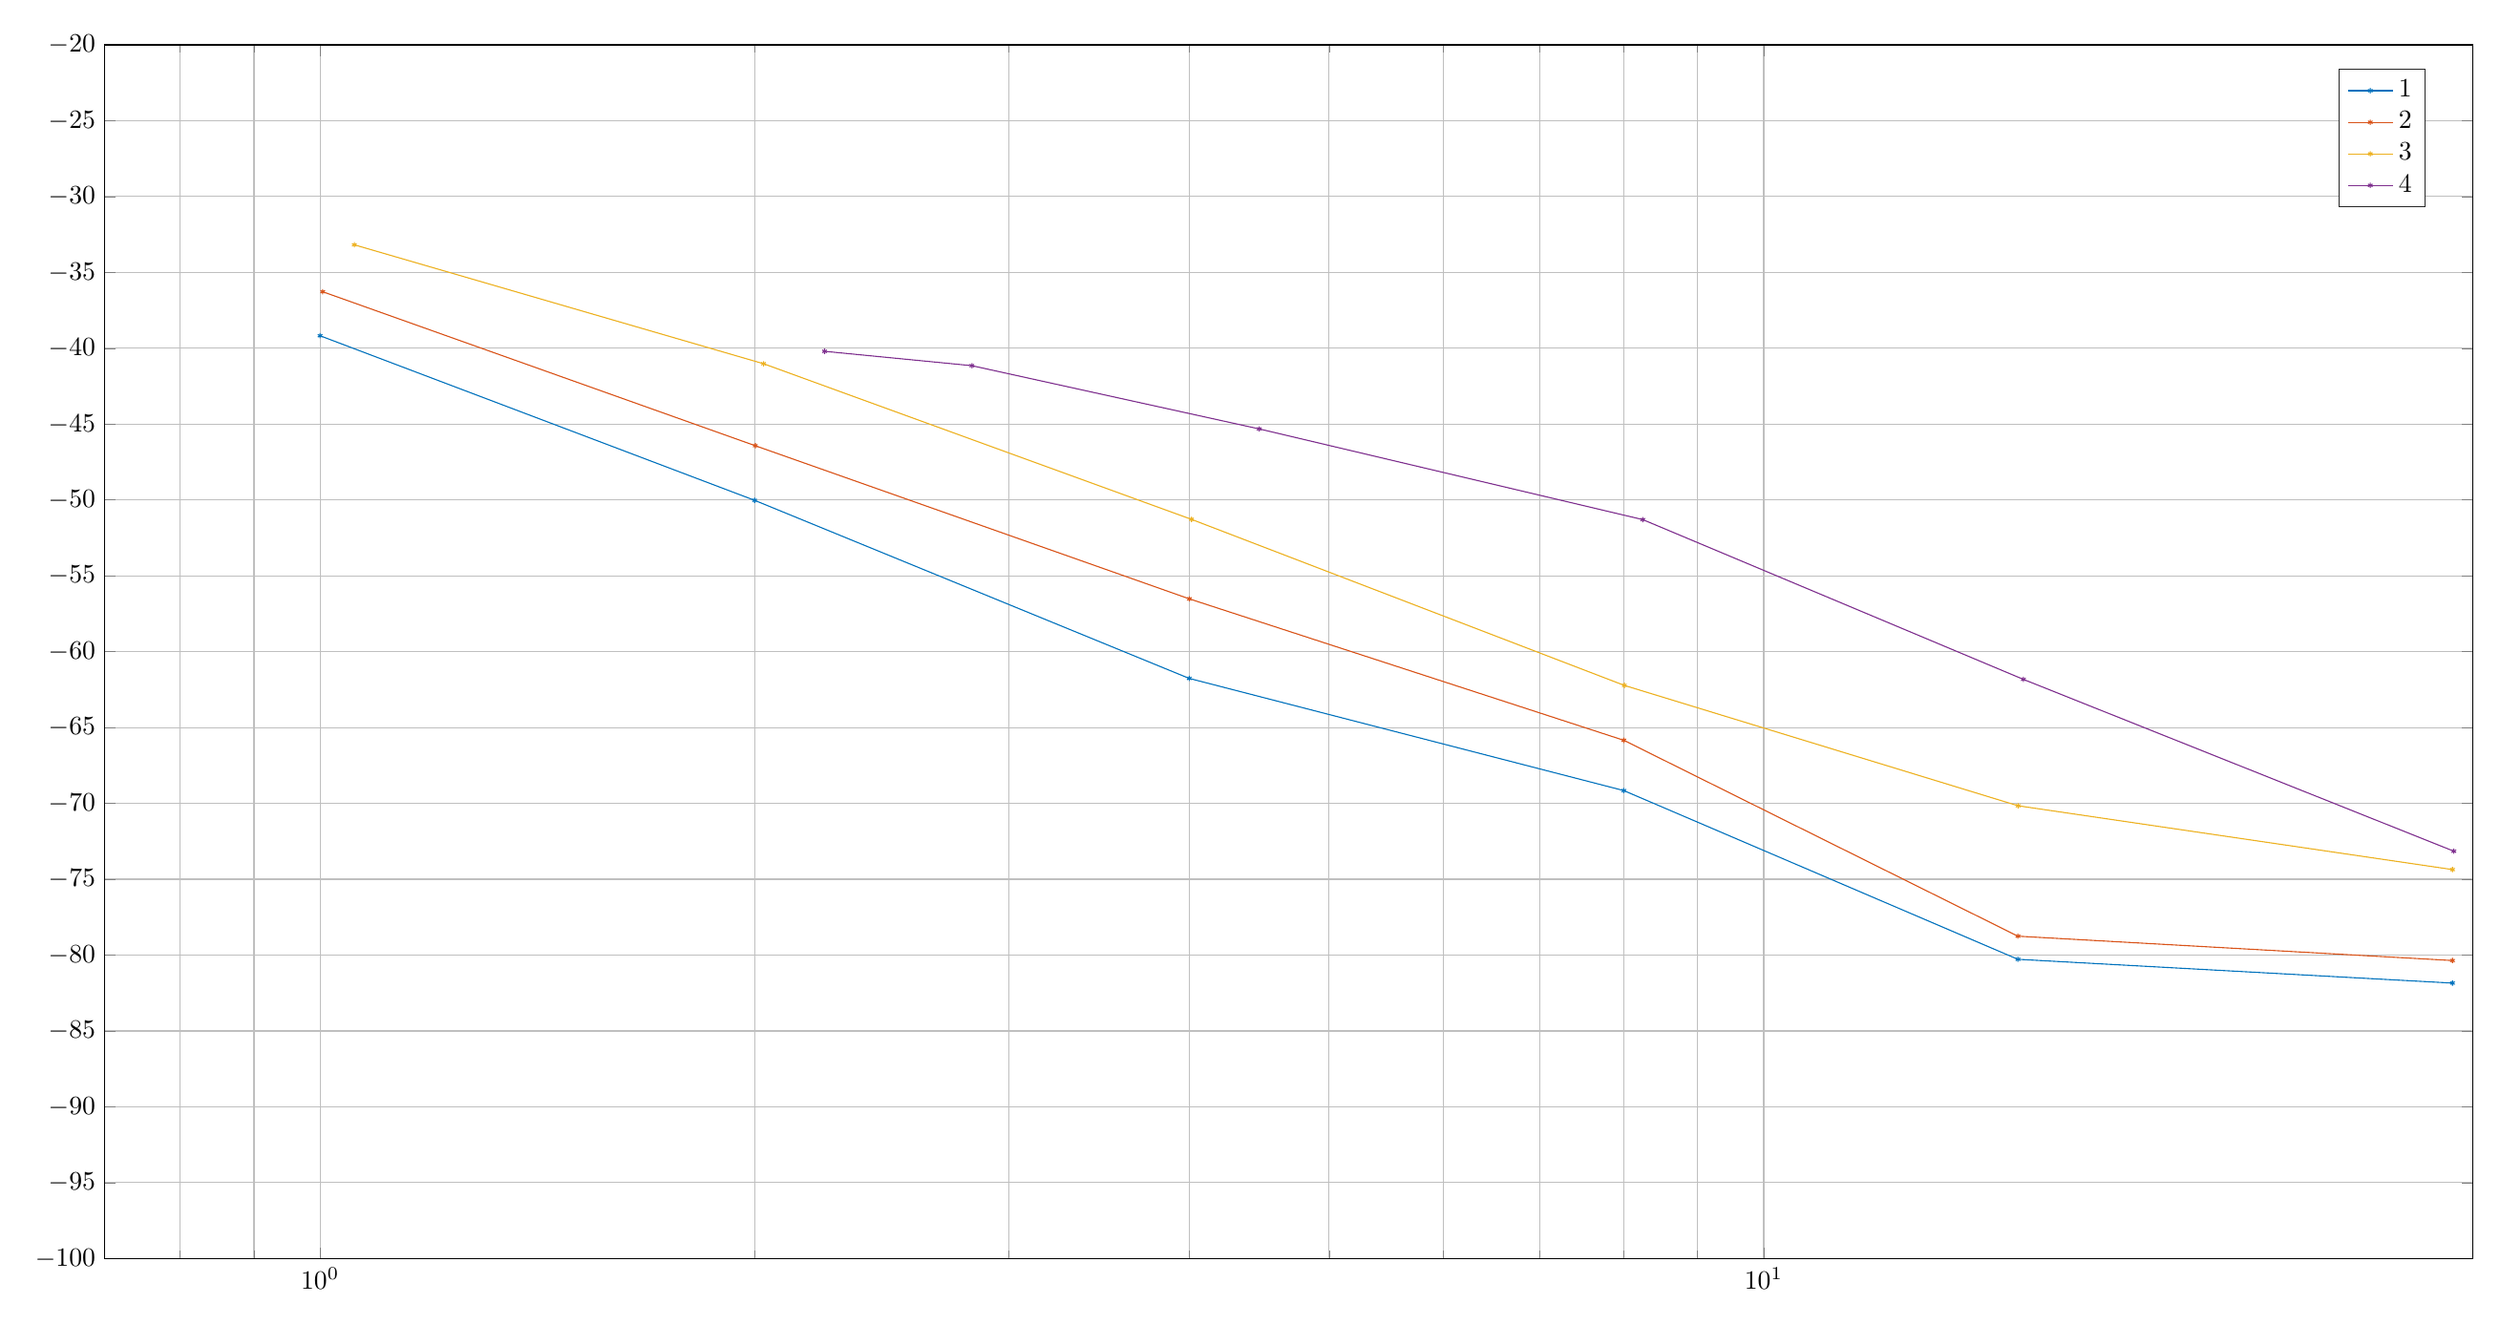
\begin{tikzpicture}

\begin{axis}[%
width=12.4in,
height=6.357in,
at={(2.08in,0.858in)},
scale only axis,
xmode=log,
xmin=0,
xmax=31,
xminorticks=true,
xmajorgrids,
xminorgrids,
ymin=-100,
ymax=-20,
ymajorgrids,
axis background/.style={fill=white},
legend style={legend cell align=left,align=left,draw=white!15!black}
]
\addplot [color=mycolor1,solid,mark size=1.0pt,mark=asterisk,mark options={solid}]
  table[row sep=crcr]{%
1	-39.176832441447\\
2	-50.0236813268286\\
4	-61.7627349006033\\
8	-69.1568155321866\\
15	-80.2784721484843\\
30	-81.8463231335614\\
};
\addlegendentry{1};

\addplot [color=mycolor2,solid,mark size=1.0pt,mark=asterisk,mark options={solid}]
  table[row sep=crcr]{%
1.00422308278589	-36.2750685665333\\
2.00211488181872	-46.4255855564945\\
4.0010578601165	-56.521087110148\\
8.00052898251109	-65.8421427417313\\
15.0002821306801	-78.7553243580291\\
30.000141066335	-80.3591753431061\\
};
\addlegendentry{2};

\addplot [color=mycolor3,solid,mark size=1.0pt,mark=asterisk,mark options={solid}]
  table[row sep=crcr]{%
1.05621967412087	-33.1826999363486\\
2.02869416127715	-41.0212571697177\\
4.01442399355125	-51.2789435665333\\
8.0072217404041	-62.2242106975379\\
15.0038528385212	-70.1578243580291\\
30.0019266048032	-74.3636753431061\\
};
\addlegendentry{3};

\addplot [color=mycolor4,solid,mark size=1.0pt,mark=asterisk,mark options={solid}]
  table[row sep=crcr]{%
2.23606797749979	-40.2024392944793\\
2.82842712474619	-41.1498149750094\\
4.47213595499958	-45.3166779228563\\
8.24621125123532	-51.29571423555\\
15.1327459504216	-61.8265071697177\\
30.0665927567458	-73.152023643832\\
};
\addlegendentry{4};

\end{axis}
\end{tikzpicture}%
\caption{Mesurements of PL for transmitter at 0.01m and receiver antenna at varying heights}
\label{Meas2}
\end{figure}

\begin{figure}
\centering
% This file was created by matlab2tikz.
%
%The latest updates can be retrieved from
%  http://www.mathworks.com/matlabcentral/fileexchange/22022-matlab2tikz-matlab2tikz
%where you can also make suggestions and rate matlab2tikz.
%
\definecolor{mycolor1}{rgb}{0.00000,0.44700,0.74100}%
\definecolor{mycolor2}{rgb}{0.85000,0.32500,0.09800}%
\definecolor{mycolor3}{rgb}{0.92900,0.69400,0.12500}%
\definecolor{mycolor4}{rgb}{0.49400,0.18400,0.55600}%
%
\begin{tikzpicture}

\begin{axis}[%
width=\myvara,
height=\myvar,
at={(2.08in,0.858in)},
scale only axis,
xmode=log,
extra x ticks={2,5,20}, 
extra x tick style={log identify minor tick positions=false},
every tick label/.append style={font=\tiny},
log ticks with fixed point,
xmin=0.9,
xmax=31,
xlabel=\tiny Distance (m),
xminorticks=true,
xmajorgrids,
xminorgrids,
ymin=20,
ymax=80,
ylabel=\tiny Path loss (dB),
title = \tiny\textbf{ht = 2.02 m},
ymajorgrids,
legend pos = north west,
axis background/.style={fill=white},
legend style={legend cell align=left,align=left,draw=white!15!black,font=\tiny}
]
\addplot [color=mycolor1,solid,mark size=1.0pt,mark=asterisk,mark options={solid}]
  table[row sep=crcr]{%
2.23606797749979	40.2024392944793\\
2.82842712474619	41.1498149750094\\
4.47213595499958	45.3166779228563\\
8.24621125123532	51.29571423555\\
15.1327459504216	61.8265071697177\\
30.0665927567458	73.152023643832\\
};
%\addlegendentry{hr = 0.04m};

\addplot [color=mycolor2,solid,mark size=1.0pt,mark=asterisk,mark options={solid}]
  table[row sep=crcr]{%
2.1541736234575	40.5286184873639\\
2.7641389255969	41.7634386176021\\
4.43175631099003	43.3569736894665\\
8.22438228683468	49.22358923555\\
15.1208618801972	58.5868821697177\\
30.060613167399	67.725648643832\\
};
%\addlegendentry{hr = 0.14m};

\addplot [color=mycolor3,solid,mark size=1.0pt,mark=asterisk,mark options={solid}]
  table[row sep=crcr]{%
1.93793704748116	37.947787309918\\
2.59915370842126	41.5490546940608\\
4.33077360294902	43.1688945864033\\
8.17041002643074	46.5688884715957\\
15.0915738079234	52.6026681377669\\
30.0458915660694	64.022898643832\\
};
%\addlegendentry{hr = 0.36m};

\addplot [color=mycolor4,solid,mark size=1.0pt,mark=asterisk,mark options={solid}]
  table[row sep=crcr]{%
1	28.6391813268286\\
2	35.8754849006033\\
4	42.4804405321866\\
8	48.4989721484843\\
15	51.0989481335614\\
30	59.847479174472\\
};
%\addlegendentry{hr = 2.02m};

\end{axis}
\end{tikzpicture}%
\caption{Mesurements of PL for transmitter at 2.00m and receiver antenna at varying heights}
\label{Meas3}
\end{figure}

In both cases, it is seen that the lower the heights of the antennas is, the higher the PL. At 